%!TEX root = main.tex
\chapter{Evaluation}
In this chapter we will describe how we evaluated the PeacefulBanana tool, and how it fulfills the requirements.

%!TEX root = main.tex
% Legger alt av usability stuff her enn så lenge

% Bruk testplan.docx og test-report.docx som en slags mal til hva som skal være med i plan og rapport. Legg det inn her 
% Se på Usability Master 2 Svanaes.pdf for et forslag til oppsett av dette. F.eks en section med gjennomføring og en med resultater. Slå sammen stuffet fra testplan.docx og test-report.docx til en fin ting!  
\chapter{Usability}
% Her bør vel det nevnes det fra testplanen, kjapt hva vi ville og resultatene stå. Vi bør også forklare testplanen mer et annet sted, såvidt i research method? Men kanskje også reintrodusere test-kapitlet og legge alt fra intro til resultater der? Bør vel ikke stå altfor mye i intro kapitlet dog
% Usability testen er jo ikke den primære evalueringen, men iom. at vi har begrenset med data bør vi nok fokusere litt på den. 
In this section we will describe the results and observations gained through usability tests. Before we conducted the usability test we created a usability test plan: Appendix \ref{chap:usability}, where all the different parts of the usability test is described in detail.
\section{Method}
The usability test was conducted on four participants. User-interaction with the PeacefulBanana was done through an Internet Browser. Users answered an entrance questionnaire, in order to collect demographic information. During the usability test we took notes of the user's problems and concerns. When the test was completed, participants could comment with suggestions on improvement of the application or design. Finally we had participants answer a SUS form, which consisted of 10 questions designed to measure user satisfaction. 

\subsection{Context}
\label{subsec:context}
The usability test simulated the two scenarios identified in Section \ref{sec:scenarios} and was set in the context of these. We conducted the usability test in order to answer several important questions, regarding these scenarios: 
\begin{itemize}
	\item Is the application easy to use, and can users achieve their goals in a timely manner?
	\item Identify the relationship users have with the aspect of reflection and sharing personal experiences.
	\item Does the tool present data in a way that triggers reflection for the user?
\end{itemize}
Feedback from the usability test was used to further aid design and help identify problem areas that might cause problems for potential users. Since the participants were all computer science experts, and familiar with reflection we hoped to collect valuable input regarding these concepts.

\subsection{Participants}
As mentioned we had four participants in the usability test. As the PeacefulBanana tool is intended to be used with developers with a computer-science background, participants were master students on the Computer Science field at NTNU. These participants all had a background from Computer Science, and were familiar with usability testing and also experienced with the notion of reflection from earlier projects using agile methodologies.
The participants' responsibilities were to attempt to complete a set of representative task scenarios presented to them in as efficient and timely a manner as possible, and to provide feedback regarding the usability and acceptability of the user interface. The participants was directed to provide honest opinions regarding the usability of the application, and to participate in post-session subjective questionnaires and debriefing.

\subsection{Procedure}
The usability test took place in a private room at the university. A computer with the PeacefulBanana web application was used in a typical working environment. The participant’s interaction with the application was monitored by the facilitator seated in the same room.
The facilitator briefed the participants on the web application and instructed the participants that are evaluating the application, rather than evaluating the participant. Participants signed an informed consent that acknowledges: \emph{the participation is voluntary, that participation can cease at any time, and that their privacy of identification will be kept safe}. \\
The facilitator explained that the amount of time taken to complete the test task will be measured and that exploratory behavior outside the task flow should not occur until after task completion. At the start of each task, the participant read aloud the task description from the printed copy and began the task. Time-on-task measurement began when the participant started the task.
The facilitator instructed the participant to ‘think aloud’ so that the facilitator could observe and take notes of user behavior and user comments.
After all task scenarios are attempted, the participant completed the post-test satisfaction questionnaire.

\subsection{Roles}
For our usability test we had two roles, in addition to the test participants: \\
\subsubsection{Facilitator}
	\begin{itemize}
		\item Provides overview of study to participants.
		\item Defines usability and purpose of usability testing.
		\item Responds to participant's requests for assistance.
	\end{itemize}
\subsubsection{Test Observer}
	\begin{itemize}
		\item Silent observer
		\item Takes notes of identified problems, concerns, coding bugs, and procedural errors.
		\item Serve as note takers.
	\end{itemize}

\subsection{Ethics}
All persons involved with the usability test were required to adhere to the following ethical guidelines:
\begin{itemize}
	\item The performance of any test participant must not be individually attributable. Individual participant's name should not be used in reference outside the testing session.
	\item A description of the participant's performance should not be reported. 
\end{itemize}

\subsection{Usability Tasks}
The usability tasks were derived from our scenarios, described in section \ref{sec:scenarios}. Due to the short time for which each participant was available, the tasks used were the most common and relatively complex of available functions. The tasks were identical for all participants in the study.
The application was tested in a development environment and databases were populated during use, and not pre-populated. This ensured a similar experience as to what the users would get when they first use PeacefulBanana in a real-life setting. The web application was run on a local computer, and not on a dedicated server as it was when deployed in production. This and the possible extra overhead from development mode, may have an impact on performance slightly in a negative way.

\subsubsection{Task context}
PeacefulBanana is a tool intended to promote reflection and allow for revisiting and learning from previous experiences. PeacefulBanana integrates with and collects data from the version-control system GitHub.
\subsubsection{Scenario 1 tasks:}
Here are the tasks participants were to solve related to Scenario 1:
\begin{itemize}
	\item Task 1: You start the application for the first time, and want to login, link your account with Github and set an active repository.
	\item Task 2: 
		\begin{itemize}
			\item Task 2.1: View your notifications.
			\item Task 2.2: Find the \emph{“Congratulations”} notification and archive it. Find the archive and see if the notification was indeed archived
		\end{itemize}
	\item Task 3:
		\begin{itemize}
			\item Task 3.1: Find the \emph{“Reminder: Daily Reflection”} note and perform the daily summary.
			\item Task 3.2: Find a daily summary note and share it. Verify that is has indeed been shared.
			\item Task 3.3: Find your mood graph
		\end{itemize}
\end{itemize}

\subsubsection{Scenario 2 tasks:}
Here are the tasks participants were to solve related to Scenario 2:
\begin{itemize}
\item Task 4:
	\begin{itemize}
		\item Task 4.1: Create a team with the name \emph{“Tuttifrutti”} and your previously chosen repository.
		\item Task 4.2: Find your created team and set it to active.
		\item Task 4.3: Identify the members on your team and their role.
	\end{itemize}
\item Task 5:
	\begin{itemize}
		\item Task 5.1: Find all your repositories’ milestones.
		\item Task 5.2: Identify your overdue milestones.
		\item Task 5.3: Find your repositories issues.
		\item Task 5.4: Find issue \#17 . Find the status of this issue, when it was opened and when it was closed.
	\end{itemize}
\item Task 6:
	\begin{itemize}
		\item Task 6.1: Generate a tagcloud for your current chosen repository.
		\item Task 6.2: Identify the most used tag for your team and yourself.
		\item Task 6.3: Find the commit impact for your repository.
	\end{itemize}
\end{itemize}

\subsection{Usability Metrics}
Usability metrics refers to user performance measured against specific performance goals necessary to satisfy usability requirements. Scenario completion success rates, error rates, and subjective evaluations was collected. Time-to-completion/Time-on-task was also collected.

\subsubsection{Task Completion}
Each task requires that the participant obtains or inputs specific data that would be used in course of a typical task. The task is noted as \emph{completed} when the participant indicates the task's goal has been obtained (whether successfully or unsuccessfully).  If a participant requires assistance in order to achieve a correct output then the task will be noted as a critical error and the overall completion rate for the task will be affected.

\subsubsection{Critical Errors}
A critical error is an error that results in an incorrect or incomplete outcome.. Obtaining or otherwise reporting of the wrong data value due to participant workflow is a critical error. Participants may or may not be aware that the task goal is incorrect or incomplete. In general, critical errors are unresolved errors during the process of completing the task or errors that produce an incorrect outcome.

\subsubsection{Non-Critical Errors}
Non-critical errors are errors that are recovered from by the participant or, if not detected, do not result in processing problems or unexpected results. Although non-critical errors can be undetected by the participant, when they are detected they are generally frustrating to the participant.

\subsubsection{Subjective Evaluations}
Subjective evaluations regarding ease of use and satisfaction was collected via questionnaires, and during debriefing at the conclusion of the session. The questionnaires utilized free-form responses and rating scales.

\subsubsection{Task Completion Time(time on task)}
The time to complete a task is referred to as "time on task", not including subjective evaluation duration. It is measured from the time the person begins the task to the time the participant indicates completion.

\subsection{Usability Goals}
The next section describes the usability goals for \emph{PeacefulBanana} in context of the usability metrics. First the general usability test objectives are described, and what usability metric results we aimed for.\\ 
The goals of usability testing the PeacefulBanana application included establishing a baseline of user performance, validating user performance measures, and identifying potential design issues that needed to be addressed in order to improve efficiency, usability and end-user satisfaction. \\
The general usability test objectives were:
\begin{itemize}
	\item Identify possible problems or breakdowns in the design\cite{ref:30} early on in the design process. Sources of such breakdowns may include:
		\begin{itemize}
			\item Navigation errors – failure to locate functions, excessive actions to complete a function, failure to follow recommended screen flow.
			\item Presentation errors – failure to locate and properly act upon desired information in screens, selection errors due to labeling ambiguities.
			\item Control usage problems – improper toolbar or entry field usage.
		\end{itemize}
	\item Exercise the PeacefulBanana application under controlled test conditions with representative users, which here are individuals with a background in IT. Data will be used to assess whether usability goals regarding an effective, efficient, and well-received user interface have been achieved.
	\item Establish baseline user performance and user-satisfaction levels of the user interface for future usability evaluations.
\end{itemize}
The PeacefulBanana application has been developed with developers in mind, and will be evaluated on students in the field of Computer Science, developing in an agile team. The testing will occur in a controlled environment in a private room.

Typical problems identified in a usability test would be text representations or the placement of design elements, that are not intuitive for the user during use. It would be a concern if the user can't figure out how to use certain features of the application. Identifying these problems as early as possible will lead to a better end design. \\
Secondly an objective of the usability test was to identify how users act and think about their daily experiences, how they react to the notion of reflecting on them and if sharing their private thoughts is a problem. 

\subsubsection{Completion Rate}
A completion rate of 100\% is the goal for each task in this usability test. \\
Completion rate is the percentage of test participants who successfully complete the task without critical errors, an \emph{output} that is correct. If a participant requires assistance in order to achieve a correct output then the task will be scored as a critical error and the overall completion rate for the task will be affected.

\subsubsection{Error-Free rate}
An error-free rate of 75\% is the goal for each task in this usability test. \\
Error-free rate is the percentage of test participants who complete the task without any errors (critical or non-critical errors). A non-critical error is an error that is not critical to get correct task output but would result in the task being completed less efficiently.

\subsubsection{Subjective Measures}
Opinions of participators regarding specific tasks, time to perform each task, features, and functionality was collected. At the end of the usability test, participants rated their satisfaction with the overall system. Combined with the interview/debriefing session. 

\subsection{Problem Severity}
In order to analyze collected data from the usability test, identified issues were classified by issue severity. This issue severity is a combination of the impact of the issue and the frequency of users experiencing the issue during the test. 

\subsubsection{Impact}
\subsubsection{Frequency}
	\begin{itemize}
		\item High: 40\% or more of the participants experienced the problem.
		\item Moderate: 20\% - 39\% of participants experienced the problem.
		\item Low: 20\% or fewer of the participants experienced the problem
	\end{itemize}
\subsubsection{Problem Severity Classification}
	\begin{itemize}
		\item High severity: High impact problems that often prevent a user from correctly completing a task. Reward for resolution is reduced redevelopment costs.
		\item Medium severity: Either moderate problems with low frequency or low problems with moderate frequency; these are minor annoyance problems faced by a number of participants. Reward for resolution is typically exhibited in reduced time on task and increased data
		\item Low severity: Low impact problems faced by few participants; there is low risk to not resolving these problems. Reward for resolution is typically exhibited in increased user satisfaction.
	\end{itemize}

\section{Usability Test Results}
\subsection{Pilot Test}
After finalizing the usability test plan: Appendix \ref{chap:usability}, a pilot test was conducted prior to the usability-test[ref 22]. The pilot test allows for an evaluation of the test plan itself and the questionaires before doing the actual usability test. This means the pilot test is a "test of the test", where the goal is to evaluate and verify that the test itself is well-formulated. We chose a fellow student as our pilot-tester, in order to check whether the test script was clear, that the tasks were appropriately difficult, and that the data collected can be meaningfully analyzed. 
It also allows the "tester" to practice the execution and guidance, before actually performing the tests. \\
In the pilot test for PeacefulBanana, all of the aspects above were evaluated and a few tweaks were made to the tests, making it more streamlined. Also a few, smaller bugs in the application were discovered and fixed. The test introduction was rewritten, since the pilot-tester showed some confusion in a few of the tasks. 
The findings acted as valuable feedback to our delivery cycle, and were used for improving the design of the application. 

\section{Summary}
We conducted an onsite usability test using a production version of PeacefulBanana, located on the test administrator’s local server. One tester took notes of comments, facial expressions and navigation choices.The administrator acted as guidance during the test. The sessions captured each participant’s navigational choices, task completion rates, comments, overall satisfaction ratings, questions and feedback.
The usability test was conducted in a private lab-room at NTNU on November 10th. The purpose of the test was to assess the usability of the web application design, information flow, information architecture and the effects of sharing personal reflection notes.
Four participants attended the test. Typically, three to five test participants is the optimal number for most usability studies\cite{nielsen1993mathematical}. Each individual session lasted approximately twenty minutes.
This section contains the participant feedback, satisfactions ratings, task completion rates, ease or difficulty of completion ratings, time on task, errors, and recommendations for improvements.
\subsection{Presentation of results}
\subsubsection{Task Completion Success Rate}
\textbf{Scenario 1 completion rates:}
\begin{figure}[h!]
    \centering
        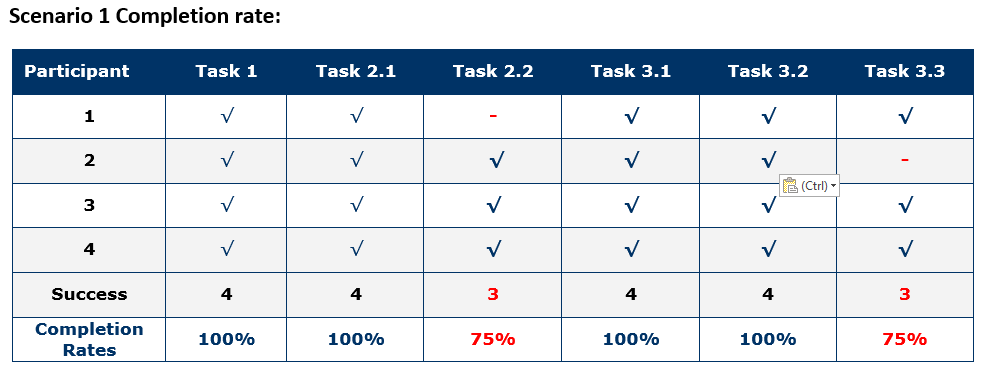
\includegraphics[width=\textwidth]{scenario1completionrate}
    \caption{Scenario 1 Completion Rate}
    \label{scenario1completionrate}
\end{figure}
\begin{figure}[h!]
    \centering
        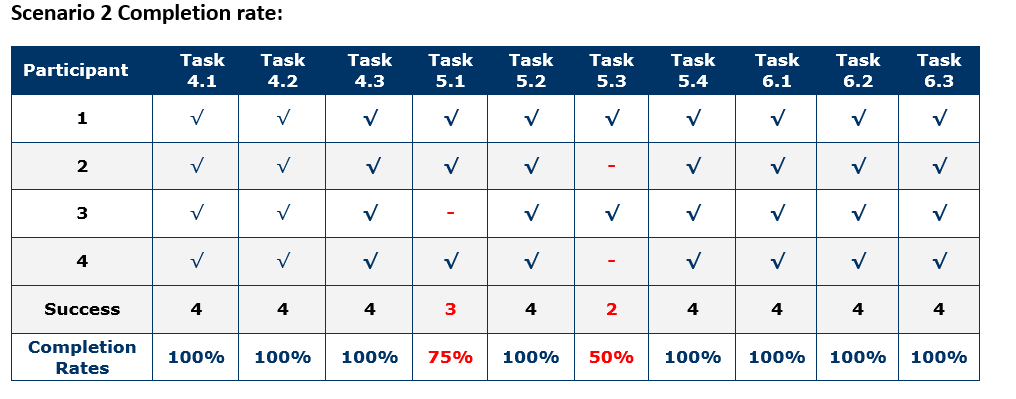
\includegraphics[width=\textwidth]{scenario2completionrate}
    \caption{Scenario 2 Completion Rate}
    \label{scenario2completionrate}
\end{figure}
All participants successfully completed (100\% Completion rate):
\begin{itemize}
	\item Task 1 - Start the application and set active repository. 
	\item Task 2.1 - View notifications. 
	\item Task 3.1 - Find the \emph{Reminder: Daily reflection} note and perform the daily summary. 
	\item Task 3.2 - Find and share the daily reflection note.
\end{itemize}
For Task 2.2(Find and archive congratulations notification) and 3.3(Find mood graph), 3 out of 4 participants completed the tasks(75\% Completion rate). \\

\textbf{Scenario 2 completion rates:}
All participants successfully completed (100\% Completion rate):
\begin{itemize}
	\item Task 4.1 - Create a team. 
	\item Task 4.2 - Set active team. 
	\item Task 4.3 - Identify team members. 
	\item Task 5.2 - Identify overdue milestones. 
	\item Task 5.4 - Find issue \#17
	\item Task 6.1 - Generate tagcloud
	\item Task 6.2 - Identify most used personal tags and team tags
	\item Task 6.3 - Find commit impact
\end{itemize}
3 out of 4 participants(75\%) successfully completed Task 5.1(Find all milestones for your repository), while 2 out 4(50\%) successfully completed Task 5.3 (Find your repositories issues). 

\subsubsection{Time on task}
Time on task for each participant was recorded. Some tasks were inherently more difficult to complete than others and is reflected by the average time on task.
\begin{figure}[h!]
    \centering
        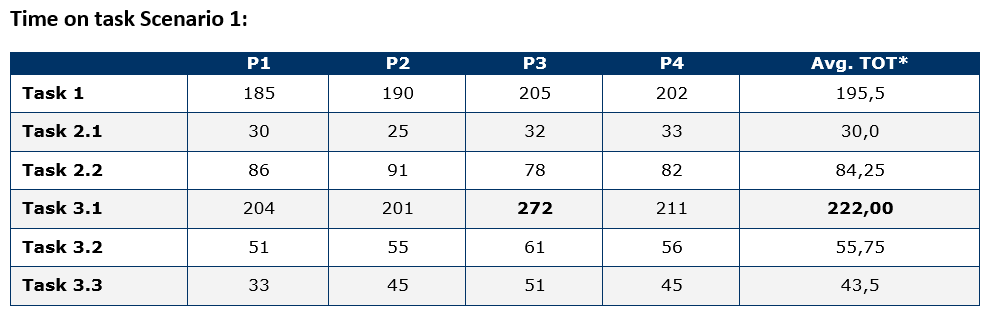
\includegraphics[width=\textwidth]{timeontaskscenario1}
    \caption{Time on task Scenario 1}
    \label{timeontaskscenario1}
\end{figure}
\begin{itemize}
	\item \textbf{Task 1(Start the application and set active team/repository)} showed a high average time on task. The main reason behind this was the authorization with GitHub which required users to login and authorize on the external GitHub.com page.
	\item \textbf{Task 2.1(View notifications)} showed a very similar time on task by the participants, the same can be seen on \textbf{Task 2.2(Find and archive notification)} although the time by each participant was over 80 seconds.
	\item \textbf{Task 3.1(Find reminder and perform daily reflection)} took the longest time to complete(average 222 seconds). However this was to be expected, as the daily reflection note requires participants to reflect on their work, and usually lasts for 2-5 minutes. This task also had the lartest range in completion time, ranging from 204 seconds to 272 seconds. \textbf{Task 3.2(Find and share reflection note)} and \textbf{Task 3.3(Find mood graph)} participant time on task averaged 55 and 43 seconds. 
\end{itemize}
\begin{figure}[h!]
    \centering
        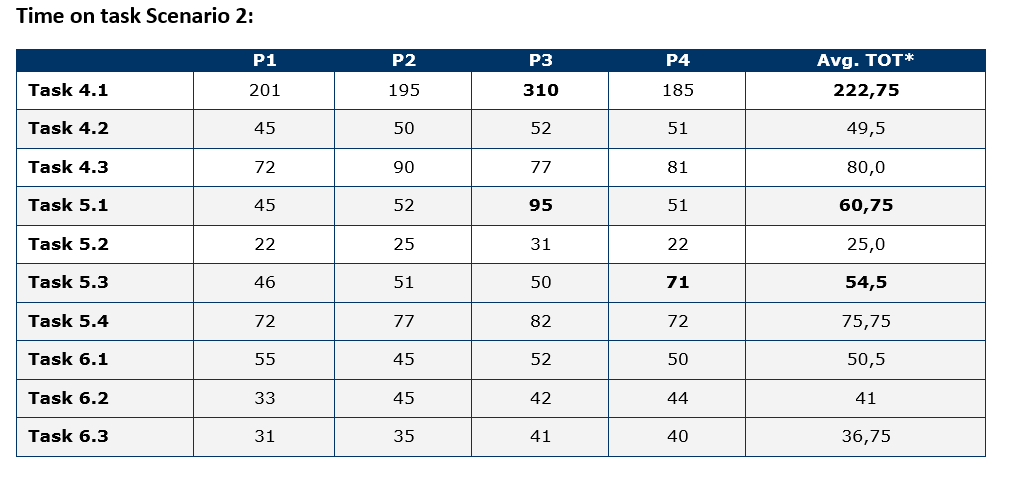
\includegraphics[width=\textwidth]{timeontaskscenario2}
    \caption{Time on task Scenario 2}
    \label{timeontaskscenario2}
\end{figure}
\begin{itemize}
	\item \textbf{Task 4.1(Create a team)} showed the longest completion time in Scenario 2. The main reason behind this was the amount of data that needed to be collected from GitHub and stored in the PeacefulBanana database. The task also showed the longest range in completion time, from 185 seconds to 310 seconds. The reason behind this large gap was mainly the difference in amount of data present in the GitHub repositories they chose to create a team for. \textbf{Task 4.2(Set active team) showed no major changes in completion time,and the same can be seen in \textbf{Task 4.3(Identify team members)}}
	\item \textbf{Task 5.1(Find all milestones)} showed that 3 out of 4 participants had very similar completion times(45, 52 and 51 seconds), but the average was increased by that the last participant had a completion time of 95 seconds. \textbf{Task 5.2(Identify overdue milestones)} showed very similar completion times, while \textbf{Task 5.3(Find repository issues)} had one participant at 71 seconds, while the rest used an average of 50 seconds. \textbf{Task 5.4(Find issue \#17)} showed an average of 75 seconds, with no signifcant differences. 
	\item \textbf{Task 6.1(Generate tagcloud)} averaged on 50 seconds, \textbf{Task 6.2(Identify most used individual and team tags)} averaged 41 seconds and \textbf{Task 6.3(Find commit impact)} averaged at 36 seconds, all with no signifcant difference in completion time. 
\end{itemize}
\subsubsection{Summary of Data}
The number of errors participants made while trying to complete the tasks were captured and recorded. Critical errors leads to participant failing in completing scenario, while non-critical errors is an error that does not prevent successful completion of the scenario. These errors along with task completions and time on task average for each task are represented in Figure \ref{datasummary}.
Low completion rate, occurance of critical-errors and high time on task are highlighted in red. 
\begin{figure}[h!]
    \centering
        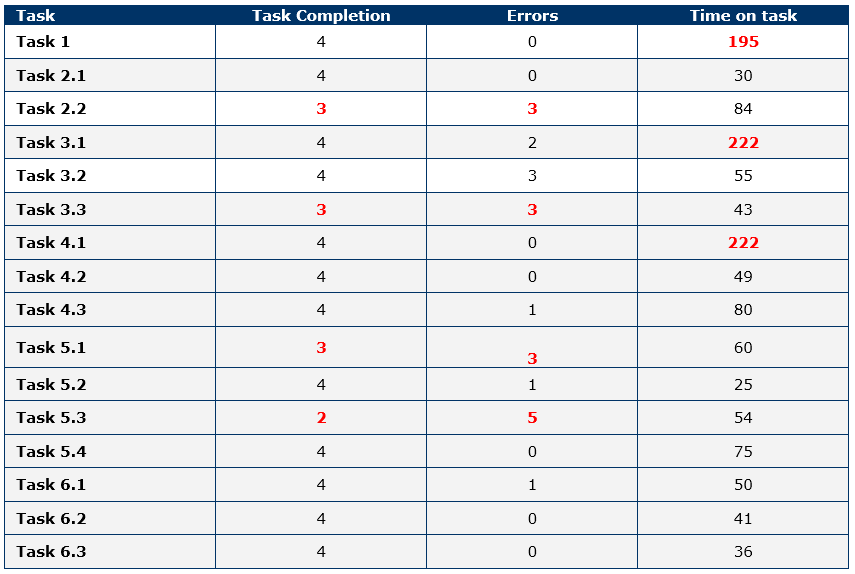
\includegraphics[width=\textwidth]{datasummary}
    \caption{Summary of Data}
    \label{datasummary}
\end{figure}

\subsubsection{Overall Metrics}
After completing the usability session, participants were given a \emph{System Usability Scale} form to answer\cite{brooke1996sus}. These can be seen in Figure: \ref{posttaskoverall}. \\

All participants agreed(i.e., agree or strongly agree) that they would use the application frequently and that the application was easy to use. All participants(100\%) also felt confident when using the application. The majority of the participants(75\%) felt the functions in the application were well integrated, and that most people would learn to use the system very qucikly. Half of the participants(50\%) agreed that there were inconsistencies in the system. None of the participants(0\%) found the system unnecessarily complex or that it was cumbersome to use. Further none of the participants felt users would need support of a technical person to use the system(based on the intended usergroup) or that they needed to learn a lot before getting going with the system. The participants mentioned the quickstart guide as a possible look-to document in case of trouble.  
\begin{figure}[h!]
    \centering
        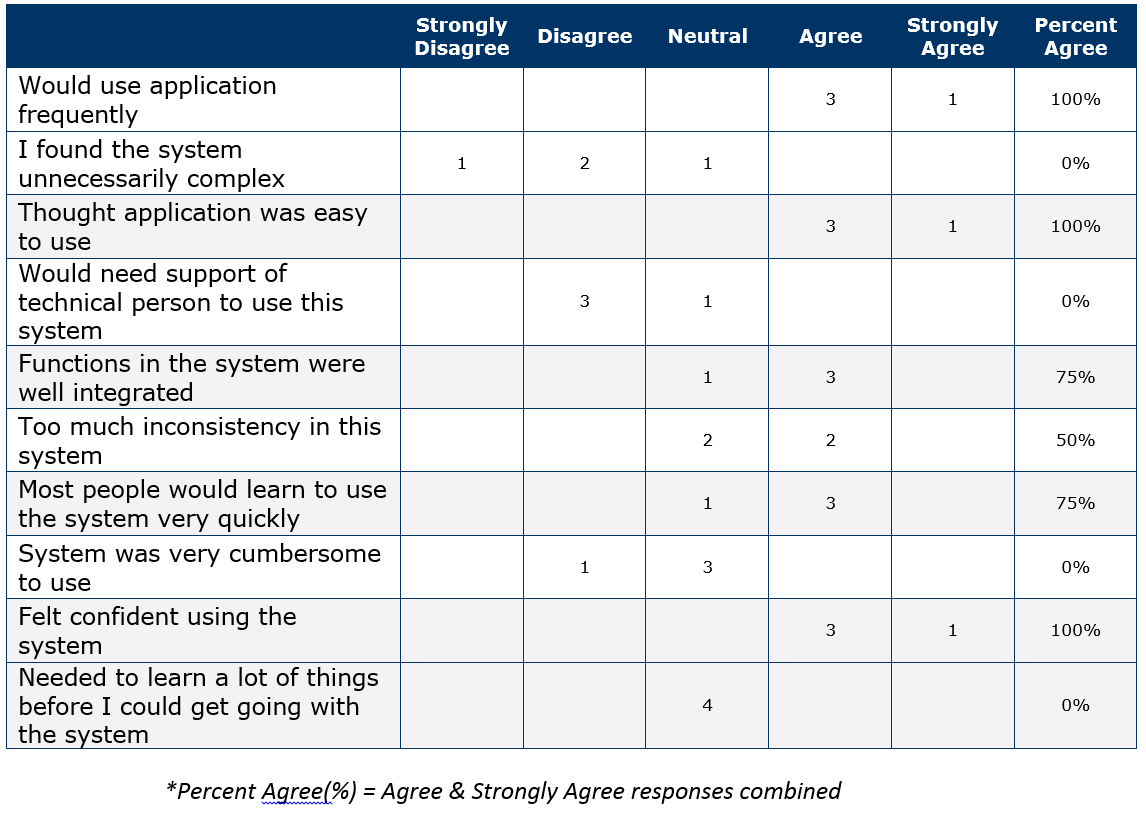
\includegraphics[width=\textwidth]{posttaskoverall}
    \caption{Post task}
    \label{posttaskoverall}
\end{figure}

\subsubsection{Reflection and sharing}
\label{subsubsec:reflection}
Participants were also asked to answer the questions identified in \ref{subsec:context}
\begin{itemize}
	\item Is the application easy to use, and can users achieve their goals in a timely manner?
\end{itemize}
Feedback here was that participants were satisfied with the ease of use as can be seen above, also time-on-task show that participants were mostly quite similar in the solving of tasks, and very few spikes. 
\begin{itemize}
	\item Identify the relationship users have with the aspect of reflection and sharing personal experiences.
\end{itemize}
On this context, participants answered that reflecting on their experiences is something they often do, but they don't collect them and thus forgets exactly what the experience was about. The application helped solve this problem by prompting and allowing users to reflect and then store it for later use. \\
When it comes to sharing, all participants were positive to this, although they strongly emphasized the need for an \emph{unshare} functionality. The missing ability to unshare these notes afterhand could make them reluctant to share them in the first place, since when first shared it was always shared. One participant mentioned the possibility of letting notes be editable and share/unshareable for a specific time period, f.ex 24 hours, where afterwards they would be locked for editing.  
\begin{itemize}
	\item Does the tool present data in a way that triggers reflection for the user?
\end{itemize}
Participants responded that the tag-cloud and questions in the daily reflection note triggered them to reflect on experiences. Actually reading the questions in their mind, helped them to reflect on the experiences, instead of just having an empty text-field could lead to random thoughts beeing collected and not actually triggering reflection. The commit impact graph was mentioned as less-helpful as it didn't really justify the amount of work done. 
	
Participants also provided feedback for what they liked the most and least about the application, and recommendations for improving the application. \\
\subsubsection*{Most liked}
The participants liked the design of the application and that it was able to synchronize with their GitHub repositories automatically, without them having to worry about it. The personal tag-cloud and the ability to compare it directly with the team's tagcloud was also a joint feedback.
\subsubsection*{Least liked}
Participants commented that the way notifications were given was not optimal, and the registration process was a bit tedious.
\subsubsection{Recommendations}
In addition to the feedback gathered from section \ref{subsubsec:reflection} above this section provides recommended changes and justifications driven by the participant success rate, behaviors, and comments. The identified recommendations will improve the overall ease of use and address the areas where participants experienced problems or found the interface/information architecture unclear.
Feedback on recommendations on improvement was primarily to streamline the registration process. Also the participants commented that issues connected to a specific milestone, should be more visibly separated from issues connected to the whole repository. \\

\subsubsection*{Add unshare functionality}
\begin{figure}[h!]
    \centering
        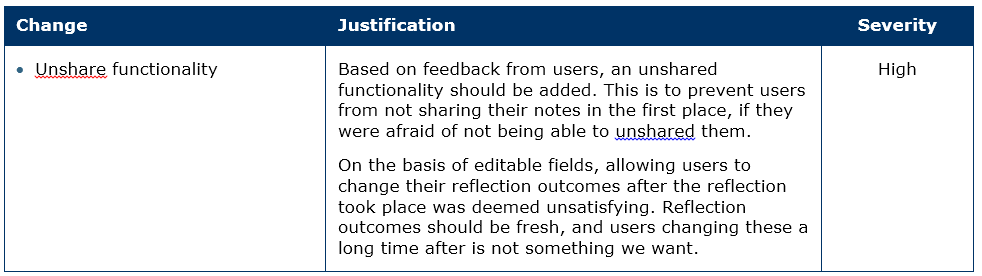
\includegraphics[width=\textwidth]{unshareimprovement}
    \caption{Adding unshare functionality to reflection notes.}
    \label{unshareimprovement}
\end{figure}

\subsubsection*{Remove commit impact}
\begin{figure}[h!]
    \centering
        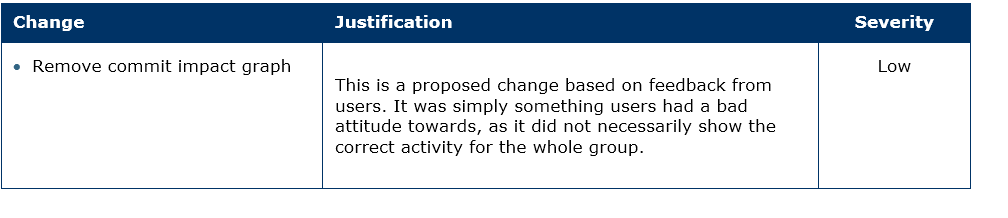
\includegraphics[width=\textwidth]{commitimprovement}
    \caption{Adding unshare functionality to reflection notes.}
    \label{commitimprovement}
\end{figure}

\subsubsection*{Task 1: Start application, login, link account with GitHub and set an active repository. } 
\begin{figure}[h!]
    \centering
        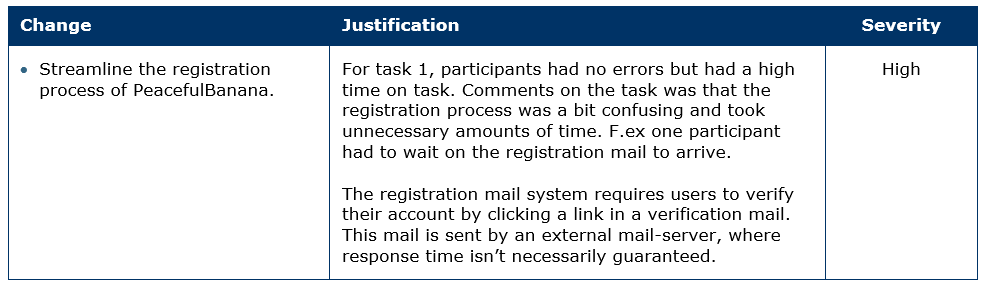
\includegraphics[width=\textwidth]{task1improvement}
    \caption{Task 1 changes and justification}
    \label{task1improvement}
\end{figure}
\subsubsection*{Task 2.2: Find the \emph{Congratulations} notification and archive it. Verify archivation.}
\begin{figure}[H]
    \centering
        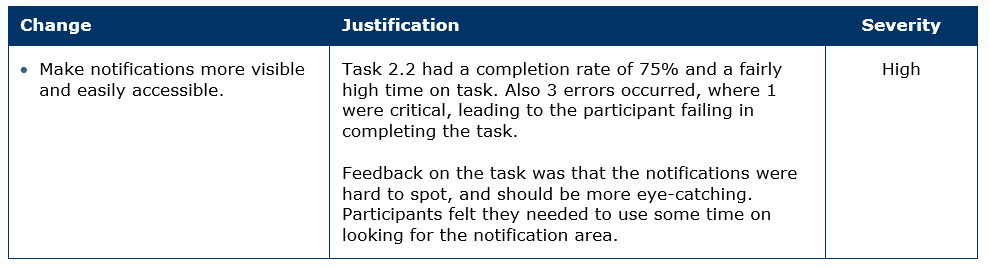
\includegraphics[width=\textwidth]{task22improvement}
    \caption{Task 2.2 changes and justification}
    \label{task22improvement}
\end{figure}
\subsubsection*{Task 3.3: Find the mood-graph.} 
\begin{figure}[h!]
    \centering
        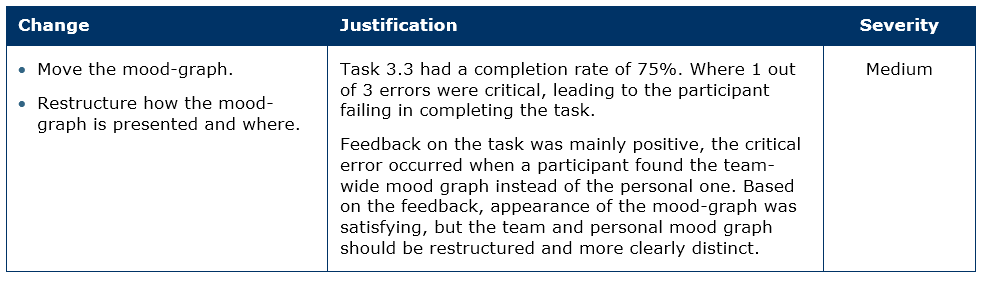
\includegraphics[width=\textwidth]{task33improvement}
    \caption{Task 3.3 changes and justification}
    \label{task33improvement}
\end{figure}
\subsubsection*{Task 5.1: Find all milestones for the current active repository.}
\begin{figure}[h!]
    \centering
        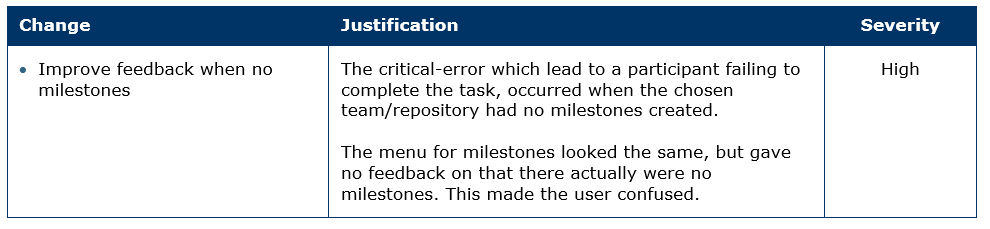
\includegraphics[width=\textwidth]{task51improvement}
    \caption{Task 5.1 changes and justification}
    \label{task51improvement}
\end{figure}
\subsubsection*{Task 5.3: Find repository related issues.} 
\begin{figure}[H]
    \centering
        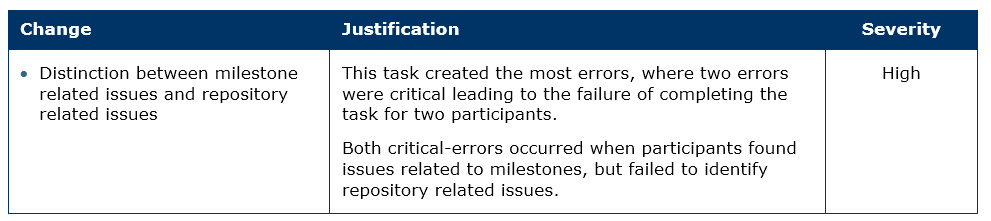
\includegraphics[width=\textwidth]{task53improvement}
    \caption{Task 5.3 changes and justification}
    \label{task53improvement}
\end{figure}

\subsection{Conclusion}
% Noe mer?
Most of the participants found the PeacefulBanana application to be well-organized, comprehensive, clean and uncluttered, very useful, and easy to use. Having an application to handle reflection in their daily work is to many if not all of the participants. Implementing the recommendations and further feedback from users will ensure a continued user-friendly application.\\
While some tasks had a high time-on-task, this was due to GitHub data collection, and is not something we have control over. It is a simple request to the GitHub API, which we need to receive before continuing. 

%!TEX root = main.tex
\section{Expert Review}
\subsection{Overview}
The expert evaluation was conducted with a senior scientist at Sintef Information and Communication Technology\footnote{Sintef ICT: \url{http://www.sintef.no/home/Information-and-Communication-Technology-ICT/}}, which also has a position as adjunct associate professor at NTNU. The evaluator is an expert in the field of agile software development and knowledge management in software companies. The evaluator has published several case studies of agile teamwork in the software development industry. He also had knowledge of version-control systems, GitHub and the use of such tools in agile development teams. Apart from the expert review, the evaluator was never directly involved in our thesis.

The evaluation performed was a type of expert walk through as described in \emph{Interaction Design - Beyond Human Computer Interaction}\citep{rogers2011interaction}. The evaluation we performed differs in that we also evaluate how the application can support agile software development teams and reflection through revisiting experiences. \\ 
The evaluation started with us presenting the main features of the application and then continued with a walk through of the application in its production state. The walk through consisted of performing the typical tasks in our scenarios. After the walk through we had an open discussion around the most common challenges agile development teams meets.  The evaluator also commented on possible shortcomings or limitations, and also any advantages the evaluator had identified in our application. We asked the evaluator to present his ideas on how our application could improve reflection in agile software development teams. We wanted an objective evaluation so we did not initially present any of our own thoughts regarding the application and its goals. \\

The evaluator suggested several possible limitations in the application, and also commented on how our application met some of the problems that often arise in development teams and how he could see our application potentially help limit these problems. We particularly went through the reflection workshop questions, to get feedback on the feasibility of these and triggering reflection in a retrospective session [See Figure \ref{workshopmandatoryexpertreview}]. 

\begin{figure}[H]
    \centering
        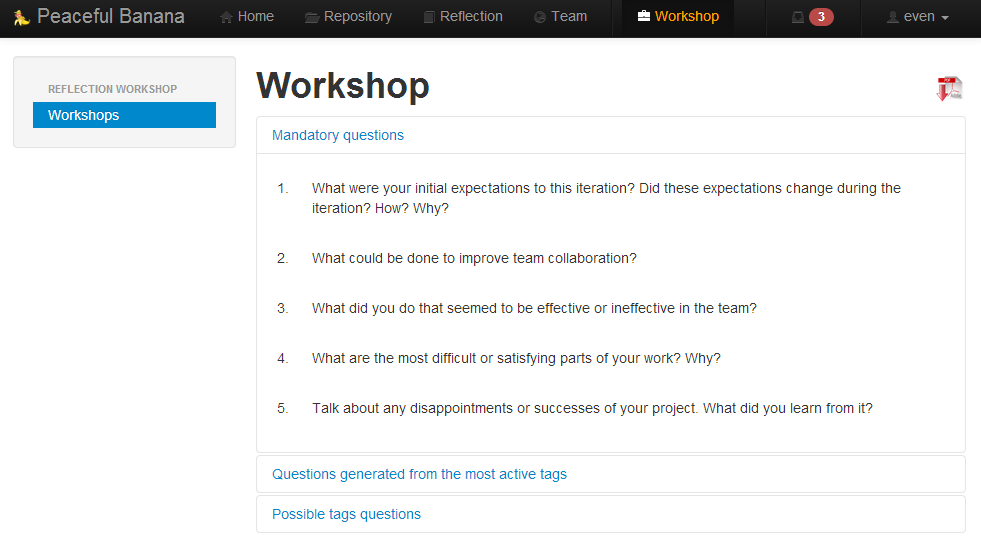
\includegraphics[width=\textwidth]{workshopmandatory}
    \caption{Example of retrospective session questions to trigger reflection.}
    \label{workshopmandatoryexpertreview}
\end{figure}

In addition to advantages and limitations of our application, the evaluator had some input towards related work he had seen, and how we could conduct the final evaluation in the best way. This included possible questions that might be relevant to ask the participants, how to get the best possible output from these and also some theory on how to analyze the results we got. \\
The feedback we got from the expert showed that the application had features that met many of the problems he had encountered through his studies of agile teams, and specifically how to trigger and enhance reflection. The evaluator also had some valuable feedback on possible shortcomings in the application, which can be typical challenges developers face in a day to day working environment. 

\subsection{Overall Feedback}
The evaluation with the Sintef expert left us with the impression that the evaluator was satisfied with the general functionality of the application, in terms of agile teams and reflection in these teams. 
At the point of evaluation, the application had been deployed to production state, and so most of the functionality was in place. The evaluator stated that the choices we had made on the data collection and representation of these was satisfying, as it allowed and encouraged users to reflect on their experiences, while not being too intrusive on the daily work routine. Both in aspects of individual and collaborative reflection the application and its functionality was satisfactory. \\

As for integration of the tool, the evaluator saw a limitation in that it was generally hard to get new tools into the daily routine of developers\citep{rogers2010diffusion}, and referred to the Technology Adoption Curve by Rogers[Figure \ref{rogerscurve}. The way we encourage users to use \#\emph{hash tags} to tag important elements in the commit message, might take some time to work in. The evaluator expressed that he was happy with the design choices made and that we chose a web-application as a platform. This way the application is available for all individuals in the team, on a wide variety of devices. This availability is important in order to further lower the threshold of usage. Apart from general feedback and app-specific feedback we also got some feedback regarding the final evaluation. Specifically what questions to ask, comparing their previous retrospective routines with a retrospective using our application beforehand. Also feedback on how to properly analyze the results we would get was valuable. The evaluator had identified possible reasons for why a certain outcome could occur through his studies. The evaluator was also pleased with the notion of allowing teams to see what notes are shared , which allowed for identification of \emph{sharing patterns} among the users. This is something that could help encourage a \emph{"discussion about reflection in the retrospective sessions"}. Another point was that individual users tend to use the same tools in different ways, so specifying what and how the application could be used before users started using the tool was important.  
\subsection{App-specific feedback}
Here we will present the challenges the evaluator presented in the aspect of teamwork and reflection in agile software development teams. The challenges identified in Table \ref{experttable} was used to create a discussion around the PeacefulBanana application and how it can solve these problems. 
\begin{figure}[H]
    \centering
        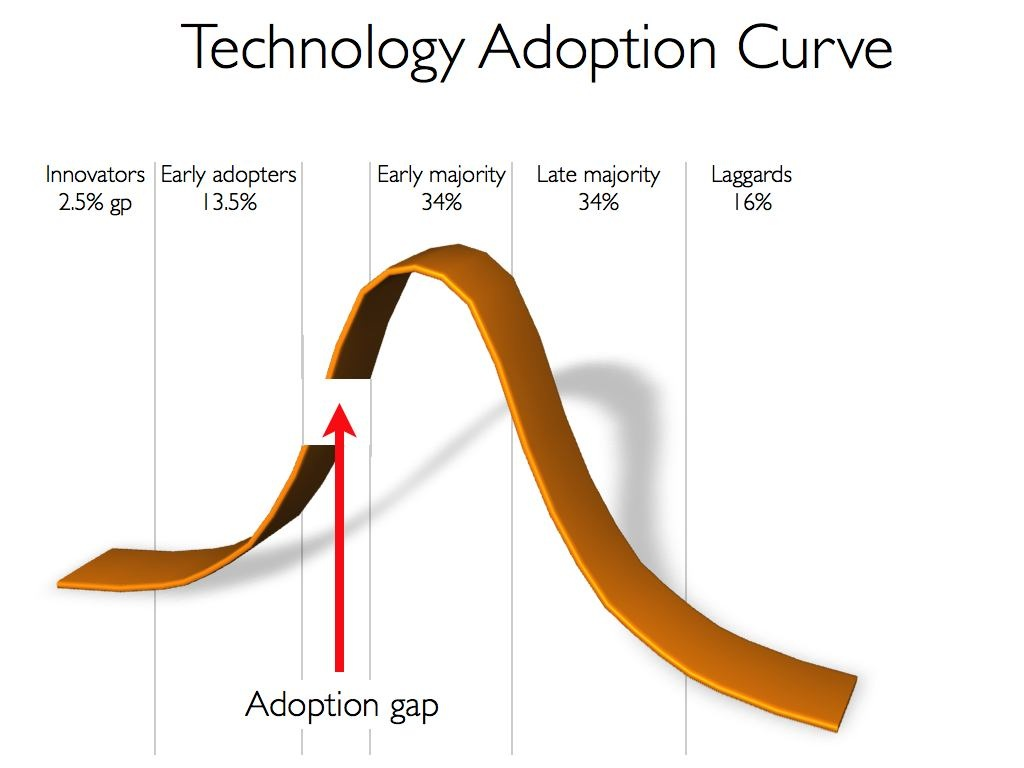
\includegraphics[width=\textwidth]{rogerscurve}
    \caption{Roger's Innovation Adoption Curve}
    \label{rogerscurve}
\end{figure}

\newpage

\begin{table}[H]
    \begin{tabularx}{\textwidth}{|l|l|X|}
    \hline
    ID & Name                & Description                                                                                                                                                                                                                                                                                                                                                    \\ \hline
    1  & Non-intrusive       & The threshold of integrating new tools into the routines of software developers is hard. The evaluator specifically referred to the \emph{Technology Adoption Curve} presented by Rogers\citep{rogers2010diffusion}, which refers to the chasm between innovators or early adopters and the early majority. This curve can be seen in Figure \ref{rogerscurve}. \\ \hline
    2  & Uniqueness          & The application should meet a demand which hasn't already been met. Also the application should provide something that a normal retrospective does not.                                                                                                                                                                                                        \\ \hline
    3  & Agile integration   & How can the application be integrated into an agile environment, helping the team to be agile and not removing the agility from the team.                                                                                                                                                                                                                      \\ \hline
    4  & Dynamic Memories    & Memories are dynamic and change over time, so there can be a lack of memorizing all important situations in a retrospective.                                                                                                                                                                                                                                   \\ \hline
    5  & Priorities          & Often agile teams develop what the developers are motivated for, and not what the customer prioritizes highest. These wrong-placed priorities can be hard to pick up.                                                                                                                                                                                          \\ \hline
    6  & Competence-overlap  & Agile teams are most efficient and deliver the highest quality work when at least two people have the same competence, so that one can ask for help and code can be reviewed by a peer. When a developer is left alone on a piece of work, integrating these parts with the rest of the project can be an issue                                                 \\ \hline
    7  & Re-work:            & Re-doing the same piece of work is also a challenge development teams can meet. When developers constantly revisits work that already has been accepted, to make unnecessary changes, the progress of the project is slowed down. Detection of this can allow for a discussion and allowing the team to progress.                                              \\ \hline
    8  & Level of expertise: & Developers often have different levels of expertise, and different areas of expertise. Even though a developer have a high amount of impact on the code-lines committed to a project, this does not mean the others don't do important work.                                                                                                                    \\ \hline
    \end{tabularx}
    \caption {Expert review feedback}
    \label{experttable}
\end{table}

\clearpage

\begin{itemize}
    \item 1. Non-intrusive:
\end{itemize}
The evaluator was satisfied with the design choice we made. By keeping the amount of time users are \textbf{required} to put into the application to a minimum, the threshold of usage is kept as low as possible at the same time. As mentioned, the Roger's adoption curve state that integrating a new tool into a daily routine is hard already, so it's important the users don't feel the application is a necessity but a helpful tool. The evaluator specifically mentioned that the daily reflection note was a good choice, since it only takes roughly 5 minutes and serves a purpose for the users. If the users then should wish to dive further into the functionality, it is easy accessible. 

\begin{itemize}
    \item 2. Uniqueness: 
\end{itemize}
The feedback here was that the evaluator had not encountered a similar tool during his research, and he felt the application met a need in the industry. As for the retrospective aspect, the feedback was that the application had features for identifying issues and situations that in a normal retrospective could be lost.  

\begin{itemize}
    \item 3. Agile integration: 
\end{itemize}
The evaluator expressed a certain concern that too much data collection could lead to an overhead in the amount of data that needed to be analyzed during the retrospective. Emphasis here was that the application shouldn't come in the way of the team being agile. 

\begin{itemize}
    \item 4. Dynamic Memories:
\end{itemize}
 The evaluator stated that by implementing the daily reflection note feature, we allowed for the most important experiences of the day being collected and stored for later use. This means that although not all data or experiences are collected, the application encourages users to reflect on fresh memories and can revisit these later during the retrospectives, hopefully omitting the risk of forgetting certain situations. 

\begin{itemize}
    \item 5. Priorities: 
\end{itemize}
The evaluator stated that this is a common problem in development teams, and thus allowing for identification of such mis-priorities are important. The feedback was that the application features for seeing how far the team has come in the particular milestones, and going into the separate issues to see when it has been worked on and by who, partially had met this challenge. The evaluator still expressed that this could be even more emphasized, and be made more easily accessible. 

\begin{itemize}
    \item 6. Competence-overlap:  
\end{itemize}
Through the different tag clouds featured in the application, a missing overlap in competence can be identified. The evaluator stated that comparing the team tag cloud with the personal tag cloud was a satisfactory way of identifying whether an individual has been working a lot alone. Further feedback was that some sort of comparing tag clouds between individuals would further help towards this challenge, but this could in turn lead to unwanted focus on individuals performance.

\begin{itemize}
    \item 7. Re-work: 
\end{itemize}
 Also here the feedback was that inspection of issues allows for seeing when and how often a problem has been fixed and then re-opened again. Also by comparing tag clouds from different periods allow for identification of much re-work. Even though the functionality was there, the evaluator wanted to make these comparisons more easily accessible in the application.

\begin{itemize}
    \item 8. Level of expertise:   
\end{itemize}
The feedback here was: Since the application focuses on project commits and comparing the users activity based on the work committed to GitHub, the application could give the wrong impression of how much work individuals in the team have done. Because of this the evaluator emphasized that we kept this fresh in mind, when describing what the tool is, what it does, what it measures and most importantly what it doesn't measure. This is important so that no users feel their work is diminished in importance by using the application.

\subsection{Suggested new features}
During our discussion with the evaluator we identified some features that were missing which could be fitting to implement in the application:
\begin{itemize}
	\item \emph{What is new?} functionality:
\end{itemize}
Show parts of the source-code in the PeacefulBanana application, creating a sort of \emph{What has happened since your last visit} functionality to the users and teams. The evaluator proposed that having such functionality might increase the user's motivation to use the application, and further trigger reflection for the daily reflection notes. 
\begin{itemize}
	\item Burn down-Chart:
\end{itemize}
The evaluator proposed including a burn down-chart based on the issues already existing on GitHub and in the PeacefulBanana application. A burn down chart is a graphical representation of work left to do versus time. The tasks or issues remaining(the backlog) is often on the vertical axis, with time along the horizontal axis.\\
A burn down chart is useful for estimating or predicting when all of the work or issues will be completed. In agile software development teams, it is a common tool to measure progress over time. The application supports some progress viewing in each milestone by presenting users with a progress bar, although the evaluator stated that a burn down-chart feature would be an addition teams would use and such increase the motivation for using the application as a whole. An example of such a burn down-chart can be seen in Figure \ref{burndownchart}. 
These features were noted as feature work, as implementing these could prove valuable for future users. 

\begin{figure}[H]
    \centering
        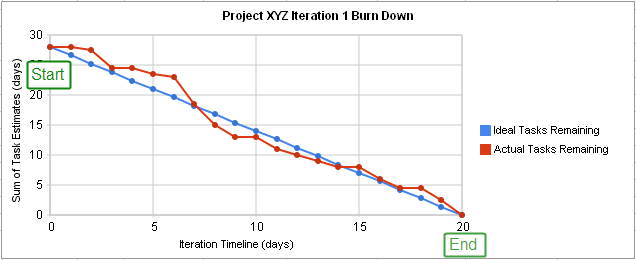
\includegraphics[width=\textwidth]{burndownchart}
    \caption{Example of a project burn down-chart}
    \label{burndownchart}
\end{figure}
\clearpage


\section{Focus group}
As a basin for the focus group interview we used \citet{FocusGrpGuide} guide on how to conduct a focus group interview. We gave the participants a smooth and snappy introduction to the agenda of the interview.

The application was evaluated with a focus group consisting of 8 NTNU students, working together in a group in the IT2901 bachelor - project. The group were using scrum as their agile project methodology, and have also used it previously in development projects. A group of 8 is fairly big, although larger focus groups are recommended in order to collect more commentaries and details from discussions\citep{morgan1998planning}. Participants in the focus group were familiar with the use of GitHub and were also using GitHub for their project at the time of evaluation. In their project they use retrospectives after each sprint, since they are using scrum. This provides the focus group with participants eager to improve their collaboration in agile teams and to improve reflection, both individually and in teams during retrospective sessions. The focus group was hosted at NTNU, in a private workshop lab with a circular table.  

The group were given the reflection scale from the MIRROR evaluation toolbox before starting the evaluation. Their answers and relationship to reflection can be seen in table \ref{reflectionscaleresults}. 
\begin{figure}[H]
\centering
	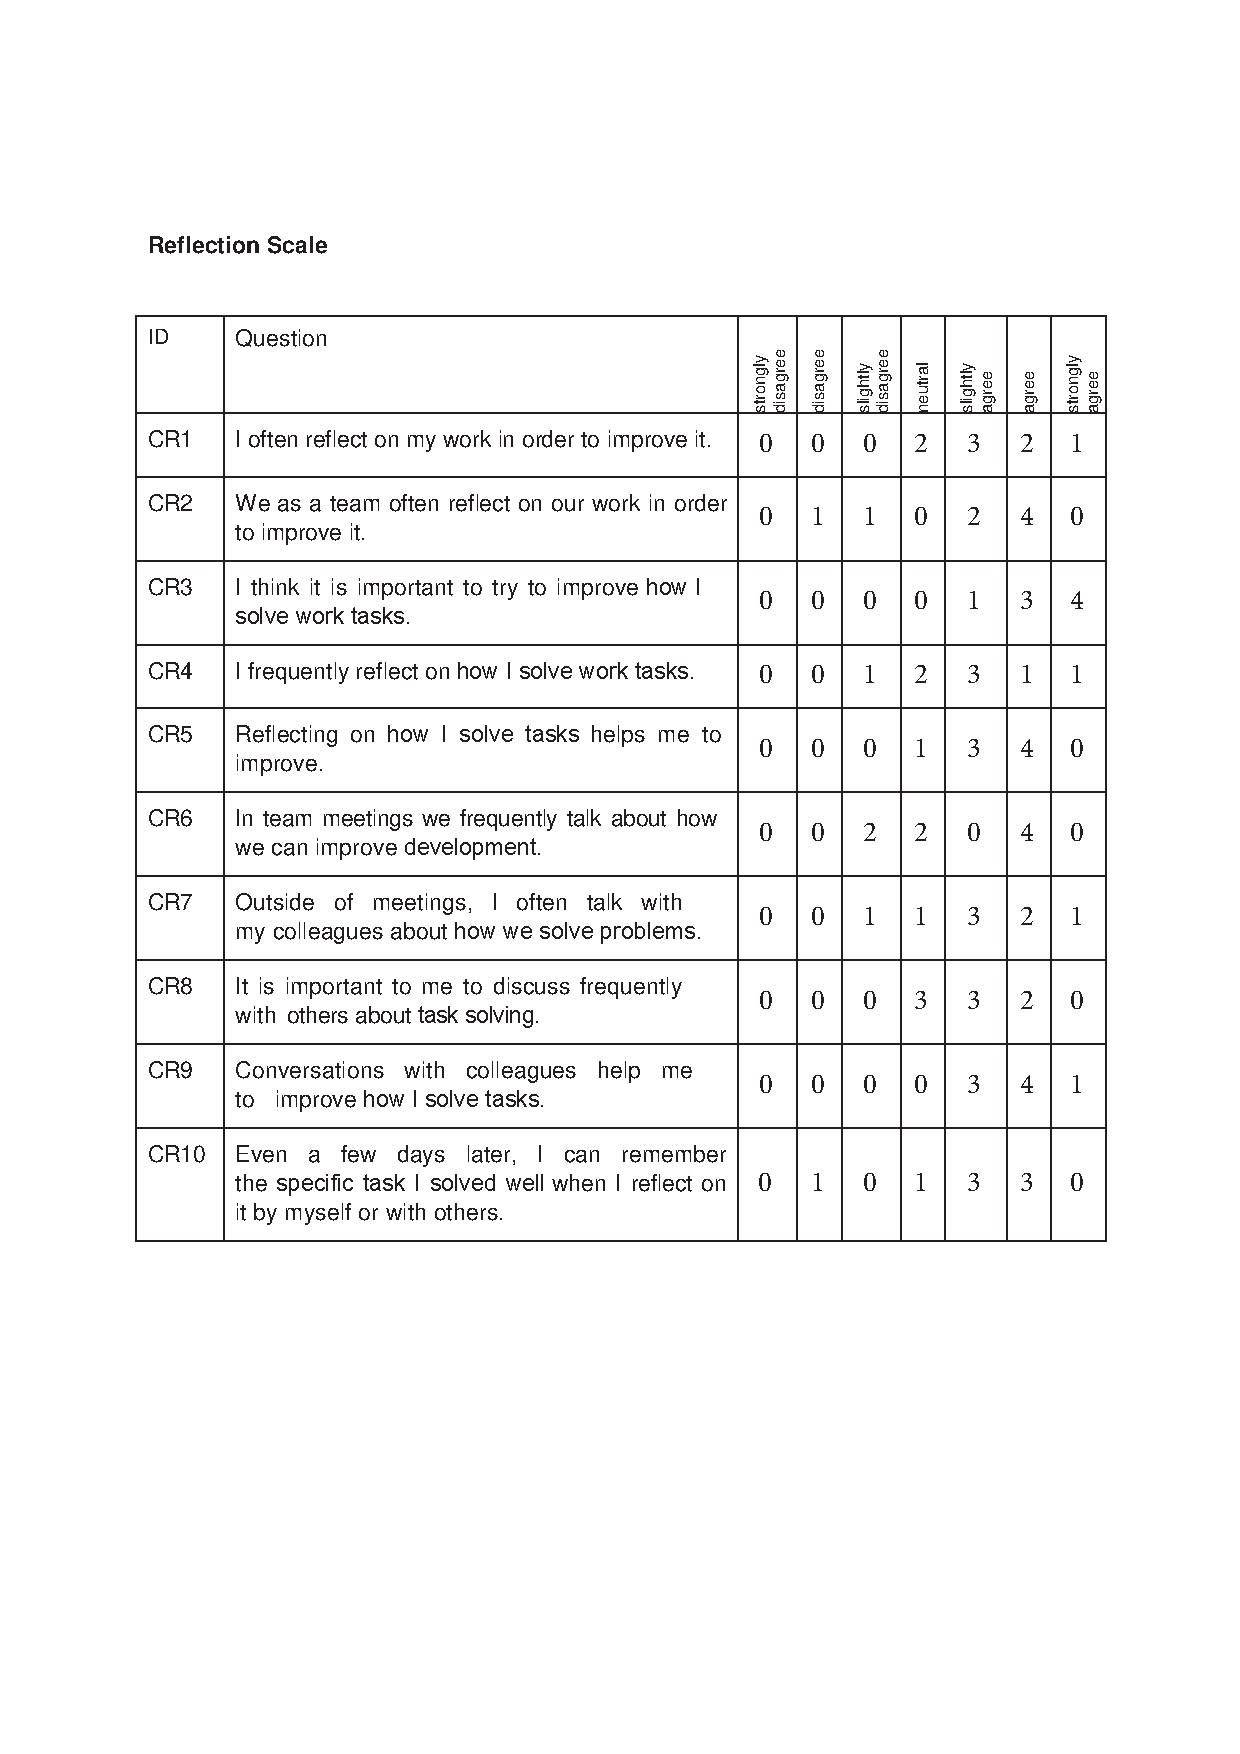
\includegraphics[width=\textwidth]{reflectionscaleresults}
\caption{Reflection scale results}
\label{reflectionscaleresults}
\end{figure}
In the table above we can see the level of agreement represented by the amount of group members which answered what for each of the questions. The group generally agree with the importance of reflection overall in the reflection scale questionnaire, however they disagree a bit with regards towards team-reflection. This is quite interesting, but during the interview we noticed a few very dominant figures in the team and this might be a the reason why the answers vary a bit when regarding team-reflection.

\subsection{Ground Rules}
In the introduction we set down a set of ground-rules that would make the interview go smoother and keep the participants distraction free. Most of these are based on the ground rules defined in \citet{FocusGrpGuide}.

\begin{enumerate}
\item Mobile phones where to be turned off during the entire interview, if you are not able to do so and receive a call. Please do this as quietly as possible.
\item We're tape recording, one person speaking at a time.
\item There is no right or wrong answer here, only opinions.
\item You don't need to agree with others, but you must listen respectfully as others share their views.
\item Talk to each other.
\end{enumerate}

\subsection{Data Collection and Analysis}
The session was recorded, in order to analyze the results after hand and also be able to participate actively during the walk through. We had prepared some application-specific questions to ask the participants during the session. These questions consisted of the most relevant app-specific questions from Section 9.1.3 in the MIRROR evaluation toolbox\citep{mirrorevaluation}. These questions were slightly modified to be used as part of the focus group and can be seen in Table: \ref{questiontable}
\begin{table}[H]
    \begin{tabularx}{\textwidth}{|l|X|}
    \hline
    1  & Can PeacefulBanana help you to collect information relevant to reconstructing experiences from work? \\ \hline
    2  & Can the application help you to reflect on experiences from work?                                    \\ \hline
    3  & Can the application help you to capture reflection outcomes?                                         \\ \hline
    4  & Does the application help you by making daily reflection notes available for later use?              \\ \hline
    5  & Does the application remind you to reflect on experiences?                                           \\ \hline
    6  & Does the application help you to find relevant experiences from others in your team?                 \\ \hline
    7  & Does the application help you to remember previous experiences and reflections?                      \\ \hline
    8  & Does the application help you to store information regarding work experiences?                       \\ \hline
    9  & Can the application help you to decide if and when to reflect?                                       \\ \hline
    10 & Do the application help you by supporting the sharing of experiences?                                \\ \hline
    11 & Does the application guide you on how to share experiences with others?                              \\ \hline
    12 & Can the application improve your collaboration?                                                      \\ \hline
    13 & Does the application provide relevant content for reflection?                                        \\ \hline
    14 & Did the application guide you through the reflection process?                                        \\ \hline
    \end{tabularx}
    \caption{}
    \label{questiontable}
\end{table}

After a brief presentation on the application itself and our goal for this thesis, the walk through started. The goal of the evaluation was primarily to see how an agile development team could integrate our tool into their daily routine. The application was evaluated with test-data, so participants could easily see how it would function in a daily work environment. After showcasing the different features, the researchers facilitated the focus group discussion on how the application could promote reflection for the team, but and also potential shortcomings or challenges to integrating it in their daily routine. The questions asked during the focus group were largely open-ended, which allowed participants freedom to express their views on the application\citep{yin2008case}. The focus group was conducted in a responsive manner, allowing us to follow up on issues uncovered mid-session and adjust the content of the focus group based on this\citep{rubin2011qualitative, wengraf2001qualitative}.

While one researcher facilitated the session, another observed and took notes, with timestamps of important parts. We swapped roles during the session, in order to prevent any variance in the notes and questioning. Any ambiguity was clarified with the participant before moving on. In order to aid analysis, the focus group was recorded and transcribed, before being analyzed. The group was also filmed so that their body-language could give us an indication about their involvement in the discussion and it was pointed out by the researchers that the interview would be anonymized to ensure that the statements could not be linked back the them.

\subsection{Why they did not use it?}
The group was intended to test use the system over a period of time, but expressed that the stress level they where under during the test period and the amount of work they had remaining made them focus on that rather than testing the tool for us. They also expressed that since the tool was made available to them so late in the process and the fact that they already had a routine worked in, they therefore forgot to include the tool in that routine on a day to day basis. The fact that they only worked a couple of days a week, which was a bit of an surprise to us as we where expecting them to work almost full-time on the project.

\subsection{If they would have used it}
When discussing tags, the group stated that they felt this might become 'off topic' and that team-members could use tags not relevant at all. This would the corrupt the tag clouds since 'off topic' tags would gain magnitude since people could use the same tags for what ever they commit ed, but when tagging issues f.ex. However one of the members expressed that he would have liked the possibility to tag an entire commit with a theme like [GUI] or [BACKBONE], the other members felt like this would been a great addition to the existing possibilities with tags.
\begin{quote}
Adding categories in brackets or something like that would put the hash tags in perspective too what people are working on and see how much time of their day goes to what part of the project. (FG1)
\end{quote}
This would then add the possibility to categories the tags in to different part of the project and we feel that this could add another dimension to the tool and help the team to see more relevance in the tags, however we feel that the themes should be decide at project-/iteration-start or at least to scaffold the themes some. This implies that the group answered yes to question 2, 3 and 8 in table \ref{questiontable} with the addendum described above which would improve the feature.

The group got had a few pointers regarding the tag cloud as well, even though the felt that it would give a good representation they felt that in order for the users to see the the relationship between the teams tag cloud and their own, tags needed to be placed at the same place and be in the same color for comparison. In the demonstration the tags where neither placed in the same place nor in the same color. 
\begin{quote}
    It is hard to locate the same tags in both of the tag clouds when they are placed in different regions of the cloud and in different color. (FG2)
\end{quote}
It was also debated whether or not it would make any difference to weight tags based on the amount of work behind the commit, but we all agreed that this could be a feature that could be implemented later. Some of the group members pointed out that even only one line changed could be just as important than an entire class.
\begin{quote}
    One line to fix a bug, can be as important or even more important than a entire new class. (FG2)
\end{quote}

They mentioned that while doing their retrospectives, they struggled to remember what they have done the week before and when discussing daily reflection notes. They felt like this would give them an new dimension to ordinary retrospectives whit the possibility to generate questions, however they had some comments on how to possibly improve the feature. By adding a text field where the user could explain what he had done that day it might enhance the level of reflection. This was something they felt was missing from project-management tools like Trello\footnote{\url{http://www.trello.com}} as they where using. When we introduced the group to the feature we call workshop preparation we where overwhelmed by the response, but they felt it could have been even better if it would have included the total tag cloud for the period selected. This gave them a possibility to reconstruct experiences recorded earlier and thus answering the question 1, 7 and 13 in table \ref{questiontable}.

As the group got closer and closer to their final evaluation they experienced that their retrospectives got shorter and shorter, it also lacked structure. When discussing the workshop-feature some of the group members commented that this could be great for a project manager that does not spend that much time with the code hands-on and in general a great tool for retrospectives, but since they had not tested the tool their was no way for them to verify it. This suggests that the group are positive to question 14 in table \ref{questiontable}.

\subsection{Comments}
%Generelle kommentarer gruppen hadde til appen
The group had some comments / suggestions on how to improve the prototype, there was one of the suggestions that we felt was essential to improve the daily reflection note feature. Instead of having the note non editable and only one each day, they suggested that we gave the users the possibility to edit the note all day and at the end of the day it will be locked so that the user can not edit it any more. This suggestion would give the user the option of noting all day long, but they will miss the feature of reflection on the days work at the end of the day as the feature was designed to do. They also suggested that the summary\footnote{With a impact cake-diagram and your own tag cloud.} should include a team tag cloud and the commits done by the user for that day.

They felt like the current notification with the daily reflection note was not enough to grab their attention and should possibly be more dominating on the site so that it was impossible to miss. This indicates that the group slightly disagreed to the question 5 in table \ref{questiontable} as they wanted the reminder to be more dominant and impossible to avoid.
\begin{quote}
The current notification is not invasive enough, it should not be possible to avoid. (FG3)
\end{quote}

It was also suggested that the group could have a meeting where they planed themes and tags for that iteration so that the tool would become more 'scrum-friendly' as they put it, when it comes to project-management. We feel that this might ensure that users visit the tool more opposite 

One of the group members said that it would be interesting to see if there is a connection on what the users are working on when they are in a bad mood, for example if a user is always unhappy when working on the GUI he should probably not work more on that part of the project.

\begin{quote}
Seems like a natural and good tool. (FG2)
\end{quote}

They also envisioned another way of using the tool as well.
\begin{quote}
I would imagine that this would be very useful for a project manager that does spend all day hands-on with coding. (FG1)
\end{quote}


\section{Discussion}
In this section we will discuss the results and experiences gathered during the usability test, expert review and focus group evaluation of the PeacefulBanana application. We will discuss this in regard of our research questions PeacefulBanana were intended to answer. We will answer all the sub research questions first, since these are more specific by trying to answer parts of the main research question. Finally we will summarize the discussion by answering the main research question, since this is the most general in terms of reflection and learning from experiences. 

\subsection{Sub RQ1}
\noindent\makebox[\linewidth]{\rule{\textwidth}{0.5pt}} 

\begin{center}
    How to scaffold collection of data in order to promote reflection? 
\end{center}

\noindent\makebox[\linewidth]{\rule{\textwidth}{0.5pt}} 
The expert evaluator expressed a concern regarding the amount of data that needed to be processed and that it should not stop the team from being agile, but also pointed out that the feature itself could help during a retrospective session. He also pointed out that the daily reflection note provided the users with a quick and easy way to reflect on a daily basis and that this would work for both users in teams and individuals. However individuals would use the functionality differently than team-users.

The focus group pointed out that they might wanted more data showed or at least the possibility to view data in their original form\footnote{Entire commit messages and issues titles in the tag cloud f.ex.} in additions to data we provided for them. They expressed that the use of commit messages to generate questions for retrospectives would give them a another dimension and more structure.

\subsection{Sub RQ2}
\noindent\makebox[\linewidth]{\rule{\textwidth}{0.5pt}} 

\begin{center}
How to increase the tendency to reflect on experiences, both individually and as a team? \\
\end{center}  

\noindent\makebox[\linewidth]{\rule{\textwidth}{0.5pt}}
Regarding the individually reflection the focus group expressed that a reminder in a tool like PeacefulBanana is a good way to trigger reflection, however they felt like the notification was a bit mild and should be more invasive to more force them to reflect over the last the 24 hours of work. Some group members expressed that the fact that the notifications needs to be read and that you can have multiple of them defeats the purpose of the notification, they are not interested in a historic overview of reflection reminders. 

They felt that the tool did not provide them with any reminder in order to improve their reflection rate as a team, however some of them stated that the link only visible to team owner and manager could have some effect in order for them to plan a retrospective session.

\subsection{Sub RQ3}
\noindent\makebox[\linewidth]{\rule{\textwidth}{0.5pt}} 

\begin{center}
How to bring together contributions from multiple users? \\
\end{center}

\noindent\makebox[\linewidth]{\rule{\textwidth}{0.5pt}}
The focus group liked that the tool had the possibility to share notes with other team members and that these notes can be inspected. The expert evaluator stated that this was vital for the users to reconstruct work experiences in order for them to reflect over past experiences. The tag-cloud could also be used to identify how much you work on different issues.
% Skrive om inspection av notes
% Tagclouds for å finne eventuelle trending issues elns


\subsection{Main RQ}
\noindent\makebox[\linewidth]{\rule{\textwidth}{0.5pt}} 

\begin{center}
How to promote experienced-based learning from reflection based on project artifacts collected from version-control systems \\
\end{center}

\noindent\makebox[\linewidth]{\rule{\textwidth}{0.5pt}} 
As discovered by the evaluation the tool gives the users the possibility to reflect over artifacts gathered from version control systems and it is shown that the evaluators find these features useful.
% Reflectere over alle de overnevte punktene over og hvordan disse svarer på 